% Options for packages loaded elsewhere
\PassOptionsToPackage{unicode}{hyperref}
\PassOptionsToPackage{hyphens}{url}
\PassOptionsToPackage{dvipsnames,svgnames,x11names}{xcolor}
%
\documentclass[
]{agujournal2019}

\usepackage{amsmath,amssymb}
\usepackage{iftex}
\ifPDFTeX
  \usepackage[T1]{fontenc}
  \usepackage[utf8]{inputenc}
  \usepackage{textcomp} % provide euro and other symbols
\else % if luatex or xetex
  \usepackage{unicode-math}
  \defaultfontfeatures{Scale=MatchLowercase}
  \defaultfontfeatures[\rmfamily]{Ligatures=TeX,Scale=1}
\fi
\usepackage{lmodern}
\ifPDFTeX\else  
    % xetex/luatex font selection
\fi
% Use upquote if available, for straight quotes in verbatim environments
\IfFileExists{upquote.sty}{\usepackage{upquote}}{}
\IfFileExists{microtype.sty}{% use microtype if available
  \usepackage[]{microtype}
  \UseMicrotypeSet[protrusion]{basicmath} % disable protrusion for tt fonts
}{}
\makeatletter
\@ifundefined{KOMAClassName}{% if non-KOMA class
  \IfFileExists{parskip.sty}{%
    \usepackage{parskip}
  }{% else
    \setlength{\parindent}{0pt}
    \setlength{\parskip}{6pt plus 2pt minus 1pt}}
}{% if KOMA class
  \KOMAoptions{parskip=half}}
\makeatother
\usepackage{xcolor}
\setlength{\emergencystretch}{3em} % prevent overfull lines
\setcounter{secnumdepth}{5}
% Make \paragraph and \subparagraph free-standing
\makeatletter
\ifx\paragraph\undefined\else
  \let\oldparagraph\paragraph
  \renewcommand{\paragraph}{
    \@ifstar
      \xxxParagraphStar
      \xxxParagraphNoStar
  }
  \newcommand{\xxxParagraphStar}[1]{\oldparagraph*{#1}\mbox{}}
  \newcommand{\xxxParagraphNoStar}[1]{\oldparagraph{#1}\mbox{}}
\fi
\ifx\subparagraph\undefined\else
  \let\oldsubparagraph\subparagraph
  \renewcommand{\subparagraph}{
    \@ifstar
      \xxxSubParagraphStar
      \xxxSubParagraphNoStar
  }
  \newcommand{\xxxSubParagraphStar}[1]{\oldsubparagraph*{#1}\mbox{}}
  \newcommand{\xxxSubParagraphNoStar}[1]{\oldsubparagraph{#1}\mbox{}}
\fi
\makeatother


\providecommand{\tightlist}{%
  \setlength{\itemsep}{0pt}\setlength{\parskip}{0pt}}\usepackage{longtable,booktabs,array}
\usepackage{calc} % for calculating minipage widths
% Correct order of tables after \paragraph or \subparagraph
\usepackage{etoolbox}
\makeatletter
\patchcmd\longtable{\par}{\if@noskipsec\mbox{}\fi\par}{}{}
\makeatother
% Allow footnotes in longtable head/foot
\IfFileExists{footnotehyper.sty}{\usepackage{footnotehyper}}{\usepackage{footnote}}
\makesavenoteenv{longtable}
\usepackage{graphicx}
\makeatletter
\newsavebox\pandoc@box
\newcommand*\pandocbounded[1]{% scales image to fit in text height/width
  \sbox\pandoc@box{#1}%
  \Gscale@div\@tempa{\textheight}{\dimexpr\ht\pandoc@box+\dp\pandoc@box\relax}%
  \Gscale@div\@tempb{\linewidth}{\wd\pandoc@box}%
  \ifdim\@tempb\p@<\@tempa\p@\let\@tempa\@tempb\fi% select the smaller of both
  \ifdim\@tempa\p@<\p@\scalebox{\@tempa}{\usebox\pandoc@box}%
  \else\usebox{\pandoc@box}%
  \fi%
}
% Set default figure placement to htbp
\def\fps@figure{htbp}
\makeatother
% definitions for citeproc citations
\NewDocumentCommand\citeproctext{}{}
\NewDocumentCommand\citeproc{mm}{%
  \begingroup\def\citeproctext{#2}\cite{#1}\endgroup}
\makeatletter
 % allow citations to break across lines
 \let\@cite@ofmt\@firstofone
 % avoid brackets around text for \cite:
 \def\@biblabel#1{}
 \def\@cite#1#2{{#1\if@tempswa , #2\fi}}
\makeatother
\newlength{\cslhangindent}
\setlength{\cslhangindent}{1.5em}
\newlength{\csllabelwidth}
\setlength{\csllabelwidth}{3em}
\newenvironment{CSLReferences}[2] % #1 hanging-indent, #2 entry-spacing
 {\begin{list}{}{%
  \setlength{\itemindent}{0pt}
  \setlength{\leftmargin}{0pt}
  \setlength{\parsep}{0pt}
  % turn on hanging indent if param 1 is 1
  \ifodd #1
   \setlength{\leftmargin}{\cslhangindent}
   \setlength{\itemindent}{-1\cslhangindent}
  \fi
  % set entry spacing
  \setlength{\itemsep}{#2\baselineskip}}}
 {\end{list}}
\usepackage{calc}
\newcommand{\CSLBlock}[1]{\hfill\break\parbox[t]{\linewidth}{\strut\ignorespaces#1\strut}}
\newcommand{\CSLLeftMargin}[1]{\parbox[t]{\csllabelwidth}{\strut#1\strut}}
\newcommand{\CSLRightInline}[1]{\parbox[t]{\linewidth - \csllabelwidth}{\strut#1\strut}}
\newcommand{\CSLIndent}[1]{\hspace{\cslhangindent}#1}

\usepackage{url} %this package should fix any errors with URLs in refs.
\usepackage{lineno}
\usepackage[inline]{trackchanges} %for better track changes. finalnew option will compile document with changes incorporated.
\usepackage{soul}
\linenumbers
\makeatletter
\@ifpackageloaded{caption}{}{\usepackage{caption}}
\AtBeginDocument{%
\ifdefined\contentsname
  \renewcommand*\contentsname{Table of contents}
\else
  \newcommand\contentsname{Table of contents}
\fi
\ifdefined\listfigurename
  \renewcommand*\listfigurename{List of Figures}
\else
  \newcommand\listfigurename{List of Figures}
\fi
\ifdefined\listtablename
  \renewcommand*\listtablename{List of Tables}
\else
  \newcommand\listtablename{List of Tables}
\fi
\ifdefined\figurename
  \renewcommand*\figurename{Figure}
\else
  \newcommand\figurename{Figure}
\fi
\ifdefined\tablename
  \renewcommand*\tablename{Table}
\else
  \newcommand\tablename{Table}
\fi
}
\@ifpackageloaded{float}{}{\usepackage{float}}
\floatstyle{ruled}
\@ifundefined{c@chapter}{\newfloat{codelisting}{h}{lop}}{\newfloat{codelisting}{h}{lop}[chapter]}
\floatname{codelisting}{Listing}
\newcommand*\listoflistings{\listof{codelisting}{List of Listings}}
\makeatother
\makeatletter
\makeatother
\makeatletter
\@ifpackageloaded{caption}{}{\usepackage{caption}}
\@ifpackageloaded{subcaption}{}{\usepackage{subcaption}}
\makeatother

\usepackage{bookmark}

\IfFileExists{xurl.sty}{\usepackage{xurl}}{} % add URL line breaks if available
\urlstyle{same} % disable monospaced font for URLs
\hypersetup{
  pdftitle={San Pedro Flood-MAR},
  pdfauthor={Travis Zalesky},
  pdfkeywords={Arizona Tri University Recharge (ATUR), San Pedro
Watershed, Managed Aquifer Recharge, Suitability Analysis},
  colorlinks=true,
  linkcolor={blue},
  filecolor={Maroon},
  citecolor={Blue},
  urlcolor={Blue},
  pdfcreator={LaTeX via pandoc}}



\draftfalse

\begin{document}
\title{San Pedro Flood-MAR}

\authors{Travis Zalesky\affil{1}}
\affiliation{1}{University of Arizona, }
\correspondingauthor{Travis Zalesky}{travisz@arizona.edu}


\begin{abstract}
Continuation of ATUR
\href{https://travisz09.github.io/ATUR-Broad-Suitability-Analysis/}{Broad
Suitability Analysis} with emphasis on San Pedro watershed. By narrowing
the focus of this analysis I hope to achieve additional progress that
will help to inform the broader analysis downstream. Methods and
analysis closely following Aloui et al. (2024)
\end{abstract}





\section{Introduction}\label{introduction}

Please see
\href{https://www.sciencedirect.com/science/article/pii/S2352801X24000602\#bib49}{Identifying
suitable zones for integrated aquifer recharge and flood control in arid
Qatar using GIS-based multi-criteria decision-making} (Aloui et al.,
2024)

\subsection{Study Area}\label{study-area}

\begin{figure}

\centering{

\pandocbounded{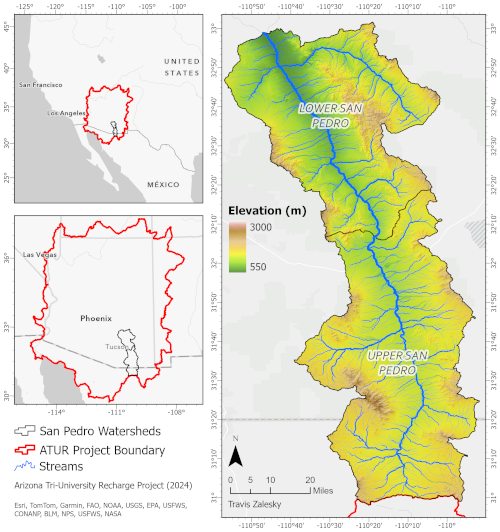
\includegraphics[keepaspectratio]{images/SanPedro_Reference_Painted.png}}

}

\caption{\label{fig-studyArea}San Pedro watershed, study area.}

\end{figure}%

\section{Data \& Methods}\label{sec-data-methods}

\subsection{Thematic Layers}\label{thematic-layers}

All data layers were processed in ArcGIS Pro v3.4.0 unless otherwise
indicated. Data layers were converted into raster data as needed, with a
30m resolution, matching the SRTM elevation raster (see
Section~\ref{sec-elev}).

\subsubsection{Elevation}\label{sec-elev}

Higher elevations are at lower flood risk due to naturally occurring
drainage, frequently in the form of surface runoff. While lower
elevations have higher surface water flow accumulation (\textbf{CITATION
NEEDED}) which can promote infiltration (\textbf{CITATION NEEDED}).

Elevation data acquired from NASA Shuttle Radar Topography Mission
(SRTM) 30m resolution global Digital Elevation Model (DEM), accessed via
Google Earth Engine (GEE) (\textbf{DATA CITATION}).

\begin{figure}

\centering{

\pandocbounded{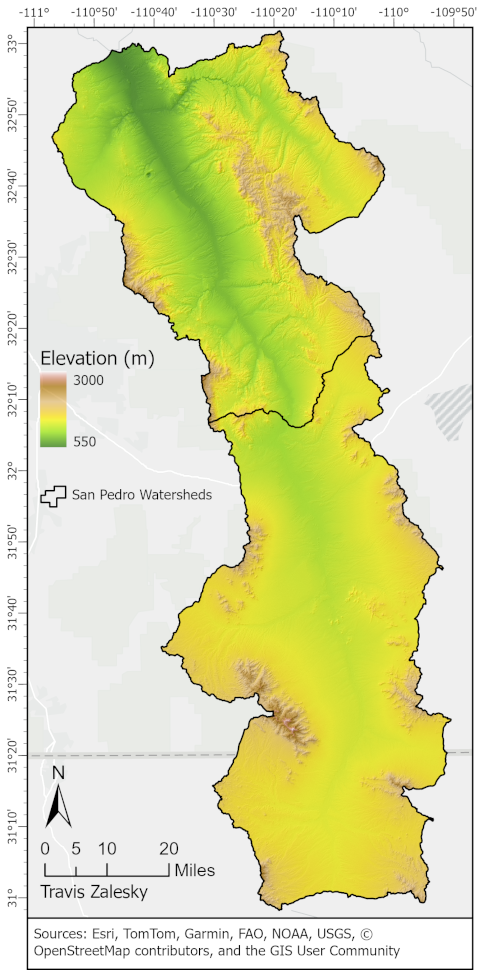
\includegraphics[keepaspectratio]{images/SanPedro_Elev.png}}

}

\caption{\label{fig-elev}San Pedro elevation 30m NASA SRTM.}

\end{figure}%

\subsubsection{Slope}\label{slope}

Steeper slopes tend to promote surface flow and high erosion. Gentler
slopes however have decreased surface water flow rates, increasing
residence time, and potentially resulting in flooding during times of
heavy rainfall or snowmelt (\textbf{CITATION NEEDED}).

Slope data was calculated as a first order derivative of the elevation
data.

\begin{figure}

\centering{

\pandocbounded{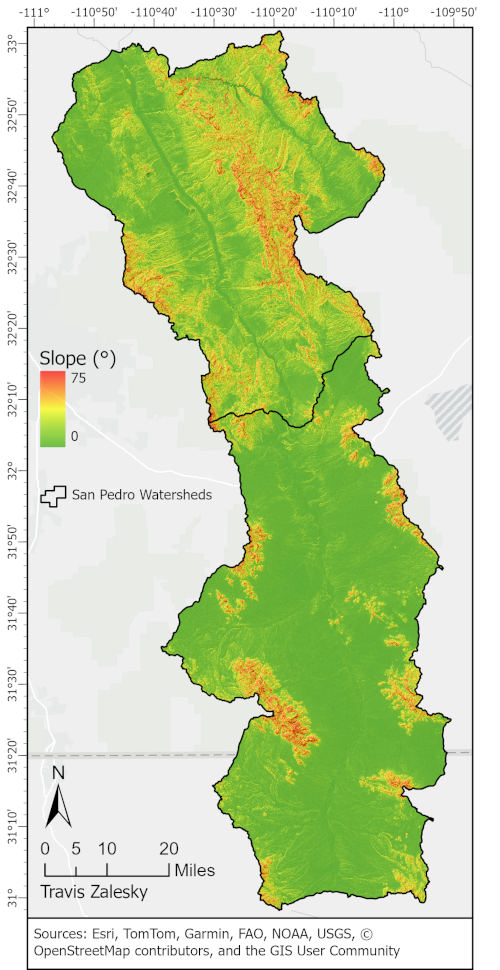
\includegraphics[keepaspectratio]{images/SanPedro_Slope.png}}

}

\caption{\label{fig-slope}San Pedro slope.}

\end{figure}%

\subsubsection{Lineament Density}\label{lineament-density}

Lineaments such as faults and fractures fundamentally influence water
flow dynamics.

\textbf{This layer is not yet available, but I believe that Ryan is
working on this concept}

See Aloui et al. (2024) section 3.1.3 Lineament density (LD) for
additional methods on generating lineament features from a DEM.

\subsubsection{Drainage Density}\label{drainage-density}

High drainage density increases flood susceptibility via rapid water
accumulation through channels (\textbf{CITATION NEEDED}). Additionally,
the increased flow rate in areas with high drainage density reduces the
residence time of surface water, limiting recharge potential
(\textbf{CITATION NEEDED}) and regions of high drainage density have
been frequently associated with less permiable soils (\textbf{CITATION
NEEDED}).

Drainage density was calculated using the USGS National Hydrography
Dataset (NHD) flowline features (\textbf{Data Citation}). This dataset
consisted of both natural and engineered flowlines, including such
things as underground pipes. Line density was calculated in Km of
flowline per Km², using a search kernel of 1 Km.

\begin{figure}

\centering{

\pandocbounded{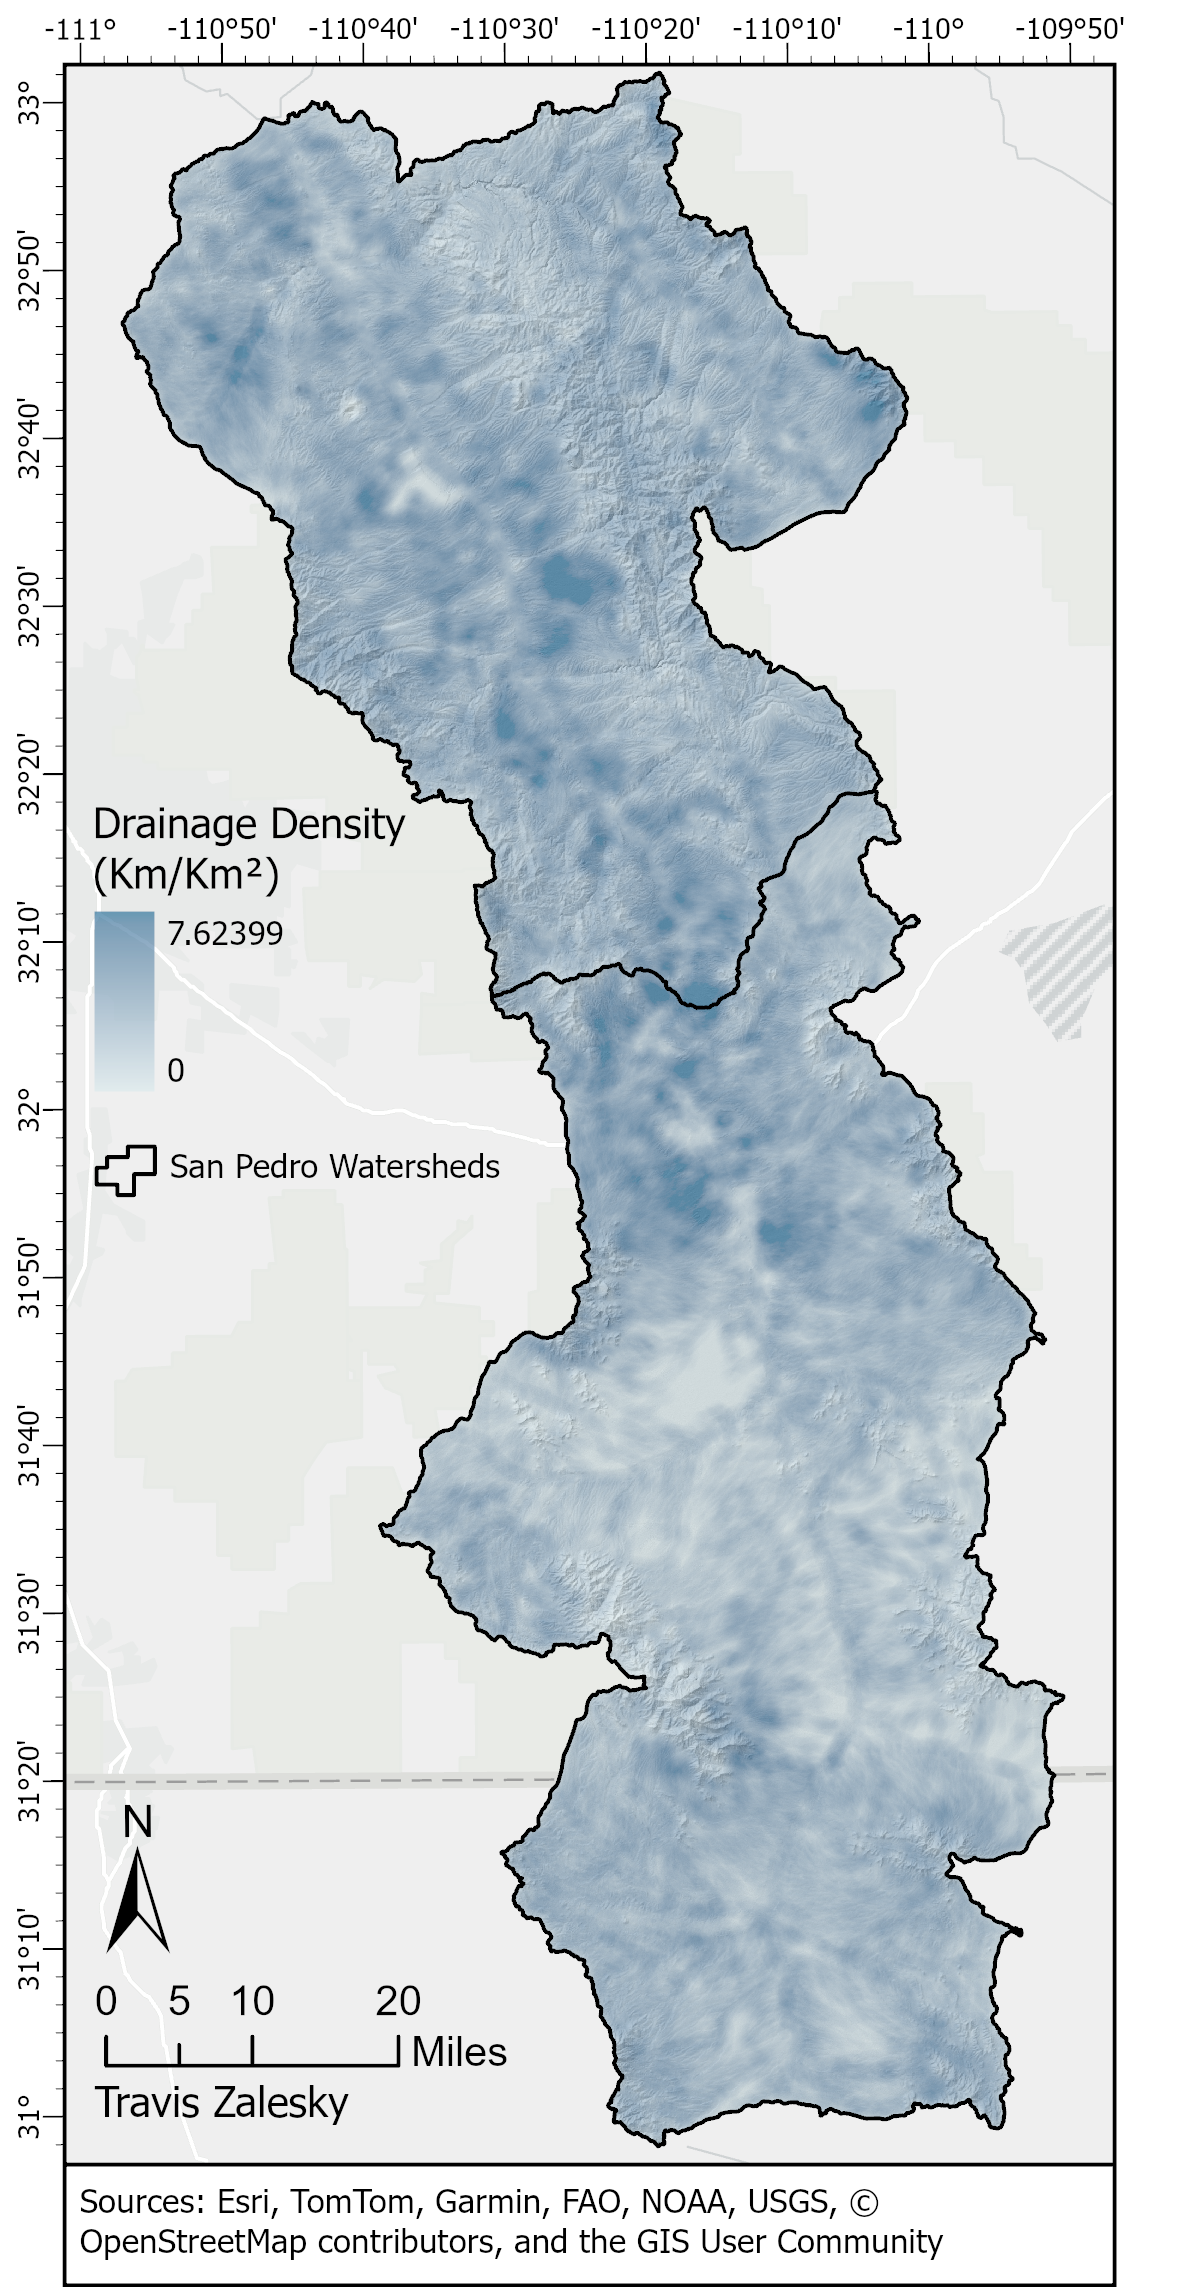
\includegraphics[keepaspectratio]{images/SanPedro_DrainDense.png}}

}

\caption{\label{fig-drain}San Pedro drainage density. Line density
calculated using a 1 Km search kernel.}

\end{figure}%

\section{Conclusion}\label{conclusion}

\section*{References}\label{references}
\addcontentsline{toc}{section}{References}

\phantomsection\label{refs}
\begin{CSLReferences}{1}{0}
\vspace{1em}

\bibitem[\citeproctext]{ref-aloui2024}
Aloui, S., Zghibi, A., Mazzoni, A., Elomri, A., \& Al-Ansari, T. (2024).
Identifying suitable zones for integrated aquifer recharge and flood
control in arid qatar using GIS-based multi-criteria decision-making.
\emph{Groundwater for Sustainable Development}, \emph{25}, 101137.
\url{https://doi.org/10.1016/j.gsd.2024.101137}

\end{CSLReferences}




\end{document}
